\begin{figure}[H]
\centering
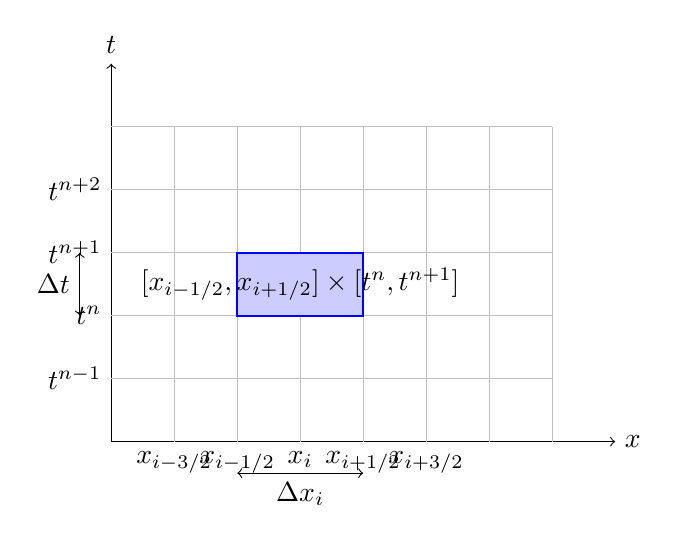
\begin{tikzpicture}[scale=0.8]
    % Draw axes
    \draw[->] (0,0) -- (8,0) node[right] {$x$};
    \draw[->] (0,0) -- (0,6) node[above] {$t$};
    
    % Draw grid lines
    \foreach \x in {1,2,3,4,5,6,7} {
        \draw[gray!50] (\x,0) -- (\x,5);
    }
    \foreach \y in {1,2,3,4,5} {
        \draw[gray!50] (0,\y) -- (7,\y);
    }
    
    % Highlight one cell
    \fill[blue!20] (2,2) rectangle (4,3);
    \draw[blue, thick] (2,2) rectangle (4,3);
    
    % Labels for the highlighted cell
    \node at (3,2.5) {$[x_{i-1/2}, x_{i+1/2}] \times [t^n, t^{n+1}]$};
    
    % x-axis labels
    \node[below] at (1,0) {$x_{i-3/2}$};
    \node[below] at (2,0) {$x_{i-1/2}$};
    \node[below] at (3,0) {$x_i$};
    \node[below] at (4,0) {$x_{i+1/2}$};
    \node[below] at (5,0) {$x_{i+3/2}$};
    
    % t-axis labels
    \node[left] at (0,1) {$t^{n-1}$};
    \node[left] at (0,2) {$t^n$};
    \node[left] at (0,3) {$t^{n+1}$};
    \node[left] at (0,4) {$t^{n+2}$};
    
    % Delta x and Delta t arrows
    \draw[<->] (2,-0.5) -- (4,-0.5) node[midway,below] {$\Delta x_i$};
    \draw[<->] (-0.5,2) -- (-0.5,3) node[midway,left] {$\Delta t$};
    
\end{tikzpicture}
\caption{Rời rạc hóa miền tính toán $\Omega$ thành các miền con}
\label{fig:domain_discretization}
\end{figure}